\documentclass[masterthesis]{fer}
\usepackage{booktabs}
% Add the option upload to generate the final version which is uploaded to FERWeb
% Dodaj opciju upload za generiranje konačne verzije koja se učitava na FERWeb


\usepackage{blindtext}
\usepackage{verbatim}


%--- THESIS INFORMATION / PODACI O RADU ----------------------------------------

% Title in English / Naslov na engleskom jeziku
\title{Emulation of Guitar Effects Using Machine Learning}

% Title in Croatian / Naslov na hrvatskom jeziku
\naslov{Emulacija gitarskih efekata primjenom strojnog učenja}

% Thesis number / Broj rada
\brojrada{1234}

% Author / Autor
\author{Luka Ivanković}

% Mentor 
\mentor{assoc. prof.\@ Domagoj Vlah, PhD}

% Date in English / Datum rada na engleskom jeziku
\date{June, 2025}

% Date in Croatian / Datum rada na hrvatskom jeziku
\datum{lipanj, 2025.}

%-------------------------------------------------------------------------------


\begin{document}


% Titlepage is automatically generated / Naslovnica se automatski generira
% \maketitle


%--- THESIS ASSIGNMENT / ZADATAK -----------------------------------------------

% Thesis assignment is included from external file / Zadatak se ubacuje iz vanjske datoteke
% Enter the filename of the PDF downloaded from FERWeb / Upiši ime PDF datoteke preuzete s FERWeb-a
% \zadatak{task.pdf}


%--- ACKNOWLEDGMENT / ZAHVALE --------------------------------------------------

\begin{zahvale}
  % Write in the acknowledgment / Ovdje upišite zahvale
  Thanks to all the giants—I did my best not to slip off the shoulders.
\end{zahvale}


% Page numbering starts from here / Odovud započinje numeriranje stranica
\mainmatter


% Table of contents is automatically generated / Sadržaj se automatski generira
\tableofcontents


%--- INTRODUCTION / UVOD -------------------------------------------------------
\chapter{Introduction}
\label{chp:introduction}

Guitar players have used pedals for a long time for more expressiveness in their songs. Effect pedals offer multiple ways to alter audio signals and change guitar tone. Traditionally, these effects are achieved through analog circuitry or digital signal processing (DSP), but designing them can be complex and time-consuming. Recently, machine learning has emerged as a promising alternative, offering the potential to emulate the sound and behavior of various guitar effects with high accuracy and less manual tuning. This thesis explores the use of machine learning techniques to model and emulate guitar effects, with the goal of achieving realistic results.

Modeling guitar effects is a technically challenging problem due to the nonlinear, dynamic, and time-dependent nature of audio transformations. Effects like distortion exhibit strong nonlinearity, while others like delay and reverb involve memory and temporal structure. 

There are three ways to approach modeling guitar effects: black-box, white-box and gray-box modeling. Black box modeling assume nothing about the internal structure of guitar effects and focus on learning end-to-end mapping straight from input to output. In contrast, white-box modeling means that every analog component needs to be meticulously measured and digitally simulated, so that the model not only produces the sounds of the modeled effect, but also allows adjusting the controls like on the modeled effect. Gray-box modeling does something in between, it tries to assume some internal structure of the modeled effect, but still relies on optimization methods to fill out unknown parameters or relationships that cannot be directly observed or derived from first principles. 

This thesis explores two of the three approaches to modeling guitar effects: black-box learning and gray-box modeling. For black-box models, we will first try out the basic fully connected network and start upgrading from there. We will introduce memory via LSTMs and later tackle more complex architectures like WaveNet, TCN, Structured state space sequence modeling. Lastly, we will try out Transformers and U-Net. These models are highly expressive and flexible but can be quite data-hungry and memory expensive, that's why the second part of this thesis will focus on gray-box optimization, more specifically, we will try out the genetic algorithm and differentiable digital signal processing and compare them to white-box modeling.

Models will be evaluated on two types of effect pedals: distortion and reverb. We will evaluate a few different loss functions and answer why training these models on a dataset without guitar recordings may also work.



%-------------------------------------------------------------------------------
\chapter{Dataset}
\label{sec:materialsandmethods}

Sound is a mechanical vibration that propagates as an acoustic wave through a medium such as air. These vibrations can be either heard by our ears which we then perceive as sound, or captured and represented digitally using audio file formats such as WAV. A standard sampling rate of 44.1 kHz means the audio signal is sampled 44,100 times per second. Why exactly 44.1 kHz is used explains Nyquist theorem, which states that to accurately reconstruct a signal, it must be sampled at least twice the highest frequency present. Since the upper limit of human hearing is approximately 20 kHz, a sampling rate just above 40 kHz is sufficient. Each sample represents the amplitude of the sound wave at a specific point in time.


The figure below \ref{fig:effects-order} illustrates a typical guitar signal chain, where the raw input from the guitar passes through an effects pedal before reaching the output (such as an amplifier or audio interface). 

\begin{figure}[htb]
  \centering
  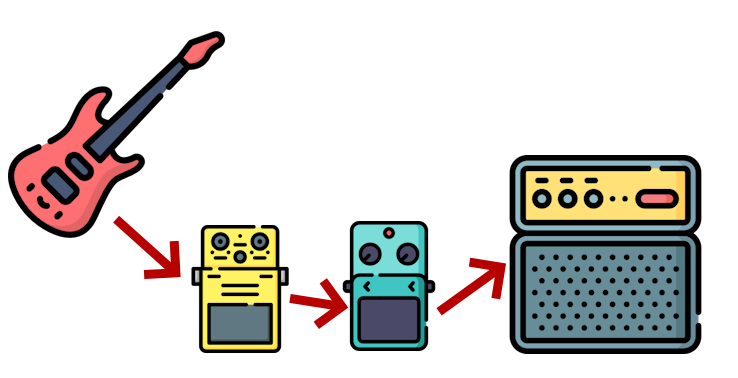
\includegraphics[width=0.6\linewidth]{Figures/audio-chain.png} 
  \caption{Typical guitar setup}
  \label{fig:effects-order}
\end{figure}

In this case, all the signals are analog, even the amplifier. The figure below \ref{fig:effects-order-2} illustrates how the same sound would be represented if captured digitally, as WAV files, before and after the pedal.

\begin{figure}[htb]
  \centering
  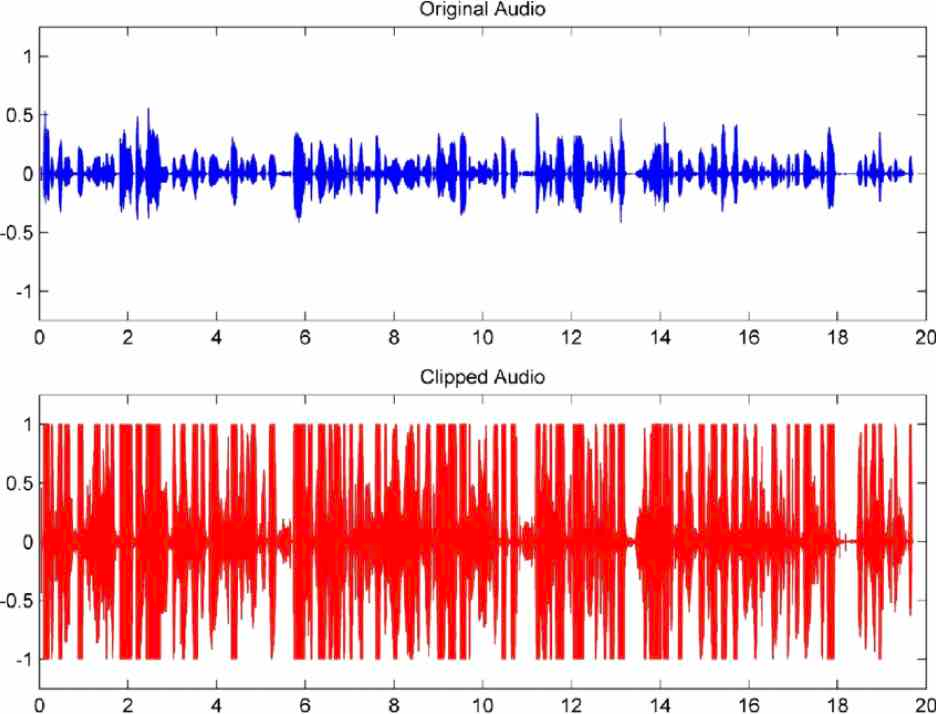
\includegraphics[width=0.5\linewidth]{Figures/effects-order-2.jpeg} 
  \caption{Audio waveform before (blue) and after (red) distortion}
  \label{fig:effects-order-2}
\end{figure}



\section{Dataset Source}
\label{sec:dataset-source}

The dataset used for this thesis is the ``Musical Instruments Sound Dataset'' by Soumendra Prasad, available on KaggleHub\footnote{\url{https://www.kaggle.com/datasets/soumendraprasad/musical-instruments-sound-dataset}}. The original dataset contains 700 recordings of guitar, drums and violin each and 528 recordings of piano with various lengths. The Test Set contains a total of 80 audio files, 20 From Each Class.

Only guitar recordings were used to train the models. Audio files in the dataset are between 1.44 and 82 seconds long. I have removed stereo files from the dataset, so only files with one channel are left. All files use 44.1 kHz sampling rate.

Since the original dataset only contains unprocessed audio files, I have applied effects on all audio files using Spotify's library PedalBoard, thus creating pairs of unprocessed and processed audio files.

\section{Effects}
Two types of effects were used in this study: \textbf{distortion} and \textbf{reverb}.
\begin{itemize}
    \item \textbf{Distortion} pedal alters an electric guitar's sound by adding gain and clipping the signal, resulting in a heavily overdriven, saturated tone, often described as "dirty" or "gritty". It's commonly used for rock and metal music to achieve a heavy, sustained sound.
    \item \textbf{Reverb} pedal simulates the natural sound reflections that occur in physical spaces, adding depth and ambience to a sound. It essentially creates the effect of playing in a room, hall, or other environment by emulating the way sound waves bounce off surfaces and decay over time. 
\end{itemize}

\subsubsection{Impulse Response}

% definition

In signal processing and control theory, an impulse response is the output of a dynamic system when presented with a very brief, idealized input signal called an impulse. Essentially, it's how a system reacts to a sudden, short change. 

\subsection{Distortion}
Memoryless distortion refers to a type of distortion in a system where the output at any given time depends only on the input at that same time, without any influence from past input values. This means the system has no memory of past inputs and its behavior is solely determined by the instantaneous input. This system corresponds to an impulse response time of 1 sample.

For simple memoryless nonlinear distortions, one can model the transformation using static nonlinear functions. An example of a simple hard-clipping distortion is:

\begin{equation}
y(t) = 
\begin{cases}
-1 & \text{if } x(t) < -1 \\
x(t) & \text{if } -1 \le x(t) \le 1 \\
1 & \text{if } x(t) > 1
\end{cases}
\end{equation}

Simple soft-clipping distortion:

\begin{equation}
y(t) = \tanh\left( g \cdot x(t) \right)
\end{equation}

In contrast to memoryless distortion, systems with memory can have output that depends on past input values. For example, a filter with a frequency response that is not flat (i.e., it affects different frequencies differently) has memory. These systems correspond to an impulse response longer than one sample.


\subsubsection{Analog vs Digital Distortion}
Analog distortion circuits rely on physical components like diodes, tubes, and transistors. These components are temperature-sensitive and may behave differently depending on humidity, power supply variation, and even the wear of the components. For instance, germanium transistors are known to sound different at different ambient temperatures.

While such small deviations are difficult to capture precisely, they generally do not significantly affect the perceptual quality.

Some pedals add non-deterministic elements, such as analog crackling or gray noise, that cannot be modeled accurately with deterministic ML systems. For example, some vintage analog fuzz pedals introduce intentional noise artifacts through unstable circuitry. Modeling such effects is theoretically impossible without modeling a stochastic source.

I opted for using simple deterministic memoryless digital distortion implemented using soft-clipping in the creation of the dataset.

\subsection{Reverb}
Reverb is a time-domain effect that simulates the natural reflections of sound in a physical space like room or hall. Unlike distortion, reverb is often linear or quasi-linear and is typically implemented as a convolution of the input signal.

Reverb is a long-memory effect, and commonly has an impulse response time of more than a few seconds. Keeping in mind that each second of audio has 44100 samples, that means the model needs to have a receptive field of 100000 samples at the very least, only to capture long-term dependencies on 3 seconds of audio. 

\subsubsection{Analog Reverb}
When digital modeling wasn't a thing, people were creative in using analog equipment to alter the sound. A good example is when they used actual springs to propagate sound. That resulted in a reverb-like effect, and it was later called spring reverb pedal and used among many guitar players. Its behavior is highly nonlinear due to the physical properties of the spring. To accurately model a spring reverb, a neural network would essentially need to approximate the behavior of a full mechanical physics engine, a task that is extremely difficult without access to the underlying physical state.

I opted for using a reverb from Spotify pedaloard. % TODO

\subsection{Other effects}

There are also modulation effects like \textbf{chorus} and \textbf{phaser}, they are typically based on dynamic time-varying parameters (e.g., low-frequency oscillators). Similarly, \textbf{compression} involves threshold-based dynamic range processing. 

These effects were chosen to be excluded, because they don't introduce a new problem % TODO
say something about all these effects being the same in terms of nonlinearity or time based as distortion and reverb

If a model is able to learn both reverb and distortion well, it is expected to be able to learn these other effects too.


\section{Chunking}

how was dataloader setup => batches and feeding chunks

what about normalization ? is dataset normalized


%-------------------------------------------------------------------------------
\chapter{Black-Box models}
\label{sec:materialsandmethods}

% TODO shorten, and add only new information in contrast to the intro where black box models were first mentioned
% references

\section{Fully Connected Networks}

% comment why FCN work on very simple distortions with minimal impulse response, but work worse on complex distortion with greater impulse response, and work terribly on reverb with even greater impulse response.
% add a table with results showing this is true

Fully Connected Networks (FCNs) are among the simplest types of neural architectures. Each neuron in a given layer is connected to all neurons in the subsequent layer. When applied to audio modeling, an FCN typically operates on short windows of the input signal.

FCNs can effectively model simple distortion effects with minimal memory — i.e., with a very short or negligible impulse response. This is because such effects are primarily nonlinear amplitude transformations, often describable by a static nonlinear function:
\[
y[n] = f(x[n])
\]
where \( x[n] \) is the input signal and \( f(\cdot) \) is the nonlinear transformation applied by the effect.

However, FCNs struggle with effects that involve longer memory, such as reverb or delay. These effects require a longer temporal context, and since FCNs do not inherently model time dependencies, they fail to capture these interactions.

Table~\ref{tab:fcn_performance} demonstrates the limitations of FCNs when modeling effects with increasing temporal complexity.

\begin{table}[h]
\centering
\caption{Performance of FCNs on Effects with Increasing Impulse Response}
\label{tab:fcn_performance}
\begin{tabular}{lccc}
\toprule
\textbf{Effect Type} & \textbf{Impulse Response Length} & \textbf{MSE Loss} & \textbf{Subjective Quality} \\
\midrule
Simple Distortion   & Short ($<$1ms)     & 0.0012 & Great \\
Dynamic Overdrive   & Medium (5–20ms)    & 0.0078 & Moderate \\
Reverb              & Long ($>$500ms)    & 0.0591 & Poor \\
\bottomrule
\end{tabular}
\end{table}



\section{Recurrent Networks (LSTM, RNN)}

%add ref to the original paper
%explain the recurrent unit briefly, and LSTM
%explain why LSTM and RNN work better than FCN on all types of pedals

Recurrent Neural Networks (RNNs) are designed to model sequential data by maintaining a hidden state that captures past information. The standard RNN was introduced in the 1980s [\cite{}], with major improvements like the Long Short-Term Memory (LSTM) architecture proposed by Hochreiter and Schmidhuber in 1997 \cite{hochreiter1997long}.

An RNN processes input sequentially:
\[
h_t = \tanh(W_{xh} x_t + W_{hh} h_{t-1} + b_h)
\]
where \( h_t \) is the hidden state at time \( t \), and \( x_t \) is the input sample.

The LSTM addresses the vanishing gradient problem inherent in vanilla RNNs, using gates to control information flow:
\begin{align}
f_t, i_t, o_t &= \sigma(W x_t + U h_{t-1} + b) \\
c_t &= f_t \odot c_{t-1} + i_t \odot \tanh(\cdot) \\
h_t &= o_t \odot \tanh(c_t)
\end{align}

Because of their memory and gating mechanisms, LSTMs and RNNs are significantly better at modeling time-dependent behaviors such as dynamic overdrive and reverberation, where past samples influence the current output. Unlike FCNs, RNN-based models can, in principle, model effects with theoretically infinite impulse responses, although in practice they often struggle to do so, mostly because of vanishing gradients. 

As it can be seen in the table~\ref{tab:lstm_performance}, LSTM performs significantly better than RNN on problems with medium impulse response, but still struggle with effects that have very long memory like reverb.


\begin{table}[h]
\centering
\caption{Comparison of LSTM and FCN on Effects with Increasing Impulse Response}
\label{tab:lstm_performance}
\begin{tabular}{lccc}
\toprule
\textbf{Effect Type} & \textbf{Model} & \textbf{MSE Loss} & \textbf{Subjective Quality} \\
\midrule
Dynamic Overdrive    & FCN     & 0.0078 & Moderate \\
Dynamic Overdrive  & LSTM    & 0.0015 & Great \\
Reverb             & FCN    & 0.0551 & Poor \\
Reverb              & LSTM    & 0.0143 & Moderate \\
\bottomrule
\end{tabular}
\end{table}


\section {Convolutional Architectures}

\subsection{WaveNet}

WaveNet, introduced by van den Oord et al. in 2016 \cite{oord2016wavenetgenerativemodelraw}, is a generative model for raw audio based on dilated causal convolutions \ref{fig:wavenet}. The model stacks layers of convolutions where the dilation factor increases exponentially, allowing the receptive field to grow without an explosion in parameters.

\begin{figure}[htb]
  \centering
  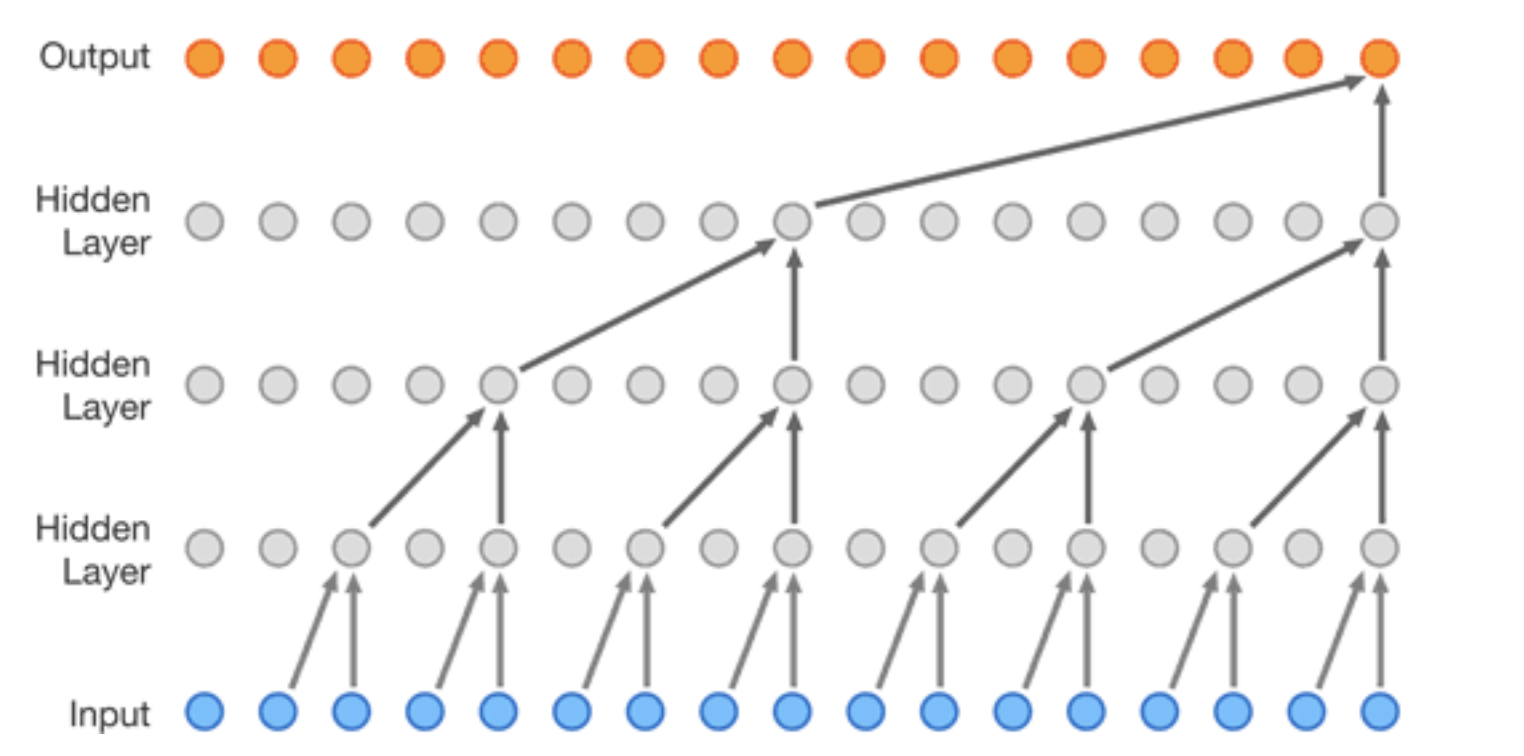
\includegraphics[width=0.6\linewidth]{Figures/wavenet_conv.png} 
  \caption{Wavenet dilated convolutions}
  \label{fig:wavenet}
\end{figure}


WaveNet is well-suited for short-term, nonlinear effects like distortion, where the output depends heavily on a small window of recent samples. However, reverb is a long-term effect with a very long impulse response, sometimes lasting several seconds, meaning the current output may depend on audio that occurred thousands or even millions of samples earlier. Because WaveNet has a finite receptive field (determined by its number of layers and dilation rates), it cannot capture such long-term dependencies effectively.

WaveNet was implemented in PyTorch with 32 residual channels, and 64 skip channels. It performed better than all previous models, but due to limited receptive field, it's impossible to model reverb or delays longer than 5 seconds. 

\begin{table}[h]
\centering
\caption{Wavenet failing to outperform LSTM on Effects with very long impulse response}
\label{tab:wavenet_performance}
\begin{tabular}{lccc}
\toprule
\textbf{Effect Type} & \textbf{Model} & \textbf{MSE Loss} & \textbf{Subjective Quality} \\
\midrule
Reverb & FCN     & 0.0078 & Moderate \\
Reverb & LSTM    & 0.0015 & Great \\
\bottomrule
\end{tabular}
\end{table}

\subsection{Temporal Convolutional Network (TCN)}

% add ref to the original paper
%comment architecture briefly
%explain why this is even better than LSTM

Temporal Convolutional Networks \cite{lea2016temporalconvolutionalnetworksaction} build upon WaveNet’s idea but introduce residual blocks and normalization. TCNs are causal, use dilated convolutions, and can model long sequences efficiently. They have the advantage of parallel computation (unlike RNNs) and avoid the vanishing gradient issues common in recurrent architectures.

Empirically, TCNs often outperform LSTMs in both convergence speed and final accuracy when modeling effects with long memory, while still retaining fast inference capabilities. They also outperform WaveNet in this task, because they do not limit receptive field to a few seconds like WaveNet does. 

 add results table


\subsection{Structured State Space Models (S4, Mamba)}

State Space Models (SSMs), Structured State Space Models 
=>  analog dynamic range compressors
%explain when S4 was first introduced add ref to the original paper
write something about mamba and how it is connected to s4
comment on results S4 vs TCN

\cite{simionato2024comparativestudystatebasedneural}



\section{Transformers}

%add ref to the original paper
%comment why transformers are not a great choice, way harder to learn, very data hungry. But they have potential

Transformers, introduced by Vaswani et al. in 2017 \cite{vaswani2023attentionneed}, revolutionized NLP by modeling global context through self-attention.


While powerful, Transformers are computationally expensive and require large datasets for effective training. Their lack of inductive bias for time locality makes them less efficient for audio applications like guitar effects emulation, especially with limited data. They also often require positional encodings to model sequential structure, which may not capture long-range dependencies as naturally as RNNs or S4.

Nevertheless, their global receptive field and flexibility make them a potential option for future work, especially in combination with more structured modules like Mamba or efficient attention variants.



\section{Generative Adversarial Networks (GANs)}

 TODO
DARKGAN?

physics-informed machine learning

%-------------------------------------------------------------------------------
\chapter{Gray-Box models}
\label{sec:graybox_models}

Gray-box models assume an existing digital signal processing chain and focus on tuning its parameters to match the behavior of a target effect. This model-based parameter optimization introduces a strong inductive bias, significantly reducing the space of possible solutions. While less flexible than black-box models, gray-box approaches are more interpretable, faster to train, and often sufficient for approximating a wide range of guitar effects.

We present two methods:
\begin{itemize}
    \item A model based on a Genetic Algorithm (GA) that searches for optimal combinations of audio effects and parameters to match a reference signal.
    \item A differentiable DSP based model that learns interpretable parameters via standard gradient optimization methods.
\end{itemize}

\section{Genetic Algorithm-Based Effect Estimation}
\label{sec:ga_model}

\subsection{Overview of Genetic Algorithms}

Genetic Algorithms are optimization techniques inspired by biological evolution. A GA operates on a population of candidate solutions, which evolve over successive generations through:
\begin{itemize}
    \item \textbf{Selection}: Favoring individuals with higher fitness (better solutions).
    \item \textbf{Crossover (Mating)}: Combining two parents to produce a new individual.
    \item \textbf{Mutation}: Introducing small random changes to maintain diversity.
    \item \textbf{Elitism}: Preserving a few top-performing individuals into the next generation.
\end{itemize}

In each generation, individuals are evaluated using a \textit{fitness function}, and the best solutions are carried forward while new candidates are generated through crossover and mutation. This process continues until convergence or a stopping criterion is reached.

%add a picture with pedals and parameters that will be optimized in algorithm

\subsection{Effect Chain Encoding and Pedalboard Integration}

We use the \texttt{pedalboard} library by Spotify to simulate common audio effects: \texttt{Compressor}, \texttt{Distortion}, \texttt{Chorus}, \texttt{Reverb}, and \texttt{Delay}. Each individual in the GA population represents a fixed sequence of these effects, with tunable parameters.

Each effect is encoded with:
\begin{itemize}
    \item A dictionary of effect-specific parameters (e.g., threshold, feedback).
    \item A \texttt{dry/wet mix} coefficient \( \alpha \in [0, 1] \), which balances unprocessed and processed audio:
    \[
    \text{output} = (1 - \alpha) \cdot \text{dry} + \alpha \cdot \text{wet}
    \]
\end{itemize}

Including the dry/wet mix greatly improves flexibility, allowing the algorithm to use subtle versions of effects.

\subsection{Fitness Evaluation and Evolutionary Process}

Each candidate effect chain is evaluated by comparing the audio it produces (by processing dry input) to a given target audio. This is done chunk-by-chunk (typically 1-second segments), and the loss is computed as the mean squared error:
\[
\mathcal{L} = \frac{1}{N} \sum_{i=1}^{N} (y_i - \hat{y}_i)^2
\]
where \( y_i \) is the target (wet) signal and \( \hat{y}_i \) is the candidate's processed output.

The population evolves according to the following steps:
\begin{enumerate}
    \item \textbf{Selection}: Tournament selection is used to choose parents. A subset of individuals compete from the old population (typically 3), and the best one is selected with high probability. Once both parents are chosen via this process, they mate and the offspring is added to the new population. The whole process repeats until the new population is as long as the old one.
    \item \textbf{Crossover}: Each child inherits one effect from either parent at each position in the chain.
    \item \textbf{Mutation}: Each effect has a chance to mutate. This may modify a parameter slightly or adjust the dry/wet mix.
    \item \textbf{Elitism}: The top 1\% of individuals (by fitness) are preserved directly into the next generation.
\end{enumerate}

The algorithm runs iteratively, logging average loss and exporting the best solution’s audio output after each generation for monitoring.

\subsection{Results and Discussion}

While this solution offers interpretability, it still fails to outperform even the basic black-box model like LSTM, and convergence is very slow due to stochastic nature of genetic algorithm. Why it fails to outperform black-box models lies in a fact that we introduced a strong inductive bias and thus limited expressivity of a model. This model can't learn the task completely unless the targeted pedal is in fact a linear combination of effects used in the algorithm. Although, assuming the problem is convex in its nature, algorithm will come as close as possible to the solution, with estimating parameters of a given effect combination (sort of like a fly trying to get as close as possible to the jam through the glass; it will reach the point on the glass where it's closest to the jam, but it's still on the glass)

 %explain briefly genetic algorithm altogether
 %explain pedalboard by spotify
 %explain the genes
 %explain the breeding
 %explain the mutation
 %explain the fitness function
 %explain why the dry wet knob was needed
 %explain tournament selection
 %
 %add results, explain why they have slow convergence



\section{Gradient-Based Optimization (DASP)}

\cite{engel2020ddspdifferentiabledigitalsignal}

DASP (it will learn faster than genetic, it's parameter space is same as genetic, that means it is limited in expressivity, although it should be "good enough" for approximating most pedals, and should learn a lot faster than regular models)

explain why both this models can't converge on pedals that can't be expressed as a linear combination of pedals inside the model. 

Paper nablafx has also mentioned the possibility to combine black box and gray box optimization, which may have potential


%-------------------------------------------------------------------------------
\chapter{Additional experiments}
\label{sec:results_and_discussion}

explain conditioning (Film, Tfilm).
we didn't need them because goal was to only find the best model that works on both reverb and distortion. Conditioning can be easily implemented if we want the parameter change in pedal and greater interpreteability.


\section{Comparison of Loss Functions}
explain spectrograms

try training with different LOSS functions (mse, spectrogram loss, ...)
why using spectrograms in loss may be benaficial, why normalizing is good for loss, and also explain why spectrograms may be slower


\section{Guitarless Dataset}
try out dataset, no guitar in  trainset, but only in valid, compare results


%--- CONCLUSION / ZAKLJUČAK ----------------------------------------------------
\chapter{Conclusion}
\label{chp:conclusion}

While the goal of this work was to provide a general model that would be good at emulating all types of guitar pedals, no such model exists with current technologies. Although some models work better on some types of effects, other models work better on other types of effects. There are tradeoffs to be made when learning a new effect, and without domain knowledge of which type of effect we are trying to emulate, it is very hard to predict which model should we choose to generalize well. 

Some complex effects might even be impossible to model with any of these methods, as they either require too much data to even approximate them well, or can't be learnt at all because of modeling complexity.

% REAL TIME MODELING explain why we dont do that here

\section{Modeling knobs}

For physical analog devices, robotic automation has become indispensable. This
method ensures precise, consistent, and repetitive adjustment of control knobs,
coupled with synchronized recording of dry input and wet output signals.
17 This
approach is crucial because manually collecting data across the continuous control
space of an amplier or pedal, with all its permutations, is oen impractical and prone
to inconsistency.
12 Robotic systems employ randomized sampling strategies over the
continuous control space, which are then optimized using pathnding algorithms
(e.g., approximations of the Traveling Salesman Problem) to minimize the total
recording time and reduce wear on mechanical components.
17 Such automated
processes can generate extensive datasets; for instance, 4.5 hours of paired audio
were collected for a single amplier model.
18

\section{Modeling LFO-based effects (Phaser, Flanger)}

A "gray-box" neural network approach has been developed using RNNs, specically
LSTMs, to model Low-Frequency Oscillator (LFO) modulated time-varying audio
eects such as phasers and angers.
16
In this approach, the network's inputs include
both the unprocessed audio signal and the LFO signal itself.
16
The explicit inclusion of the LFO signal as an input to RNNs for time-varying eects
represents a clever "gray-box" strategy that causally improves model performance
and interpretability. By directly providing the LFO signal, the model's complexity is
signicantly reduced because it is not required to learn the LFO's complex shape and
frequency from the raw audio training data.
16 This ooads a challenging estimation
task from the neural network, allowing it to focus more eectively on learning the core
transformation of the eect. Furthermore, this design choice provides a direct,
controllable parameter for the LFO aer the model has been trained, which is crucial
for musicians who need to adjust the eect's modulation rate.
16 This causal design
leads to higher accuracy, as evidenced by very low Error-to-Signal Ratios (ESR)
reported for these models: 0.2% for phasers and 0.3% for angers.
16 Errors of this
magnitude are generally considered inaudible, indicating a high level of delity.
16 The
model architecture is also capable of running in real-time on modern computing
hardware with relatively low processing power.
16


%--- REFERENCES / LITERATURA ---------------------------------------------------

% References are automatically generated from the supplied .bib file / Literatura se automatski generira iz zadane .bib datoteke
% Enter the name of the BibTeX file without .bib extension / Upiši ime BibTeX datoteke bez .bib nastavka
\bibliography{references}



%--- ABSTRACT / SAŽETAK --------------------------------------------------------

% Abstract in English
\begin{abstract}
  Enter the abstract in English.
   
\end{abstract}

\begin{keywords}
  the first keyword; the second keyword; the third keyword
\end{keywords}


% Sažetak na hrvatskom
\begin{sazetak}
  Unesite sažetak na hrvatskom.

\end{sazetak}

\begin{kljucnerijeci}
  prva ključna riječ; druga ključna riječ; treća ključna riječ
\end{kljucnerijeci}



%--- APPENDIX / PRIVITCI -------------------------------------------------------

% All following chapters will be denoted with an appendix and a letter / Sva poglavlja koja slijede će biti označena slovom i riječi privitak
\backmatter

\chapter{The Code}



\end{document}
